\documentclass{article}
% pre\'ambulo

\usepackage{lmodern}
\usepackage[T1]{fontenc}
\usepackage[spanish,activeacute]{babel}
\usepackage{mathtools}
\usepackage{graphicx}

\title{Ejercicio 1}
\author{Mar\'ia de los \'Angeles Rodr\'iguez Vela}

\begin{document}
Find the power set R3
of R = {(1, 1),(1, 2),(2, 3),(3, 4)}. Check your answer with the script powerrelation.m and write a LATEX document with the
solution step by step.

$R^2 = \{(1,1),(1,2),(1,3),(2,4)\}$

$R^3 = R^2 * R$

$R^3 = \{(1,1),(1,2),(1,3),(1,4)\}$


\maketitle

Mi primer documento en \LaTeX{}.

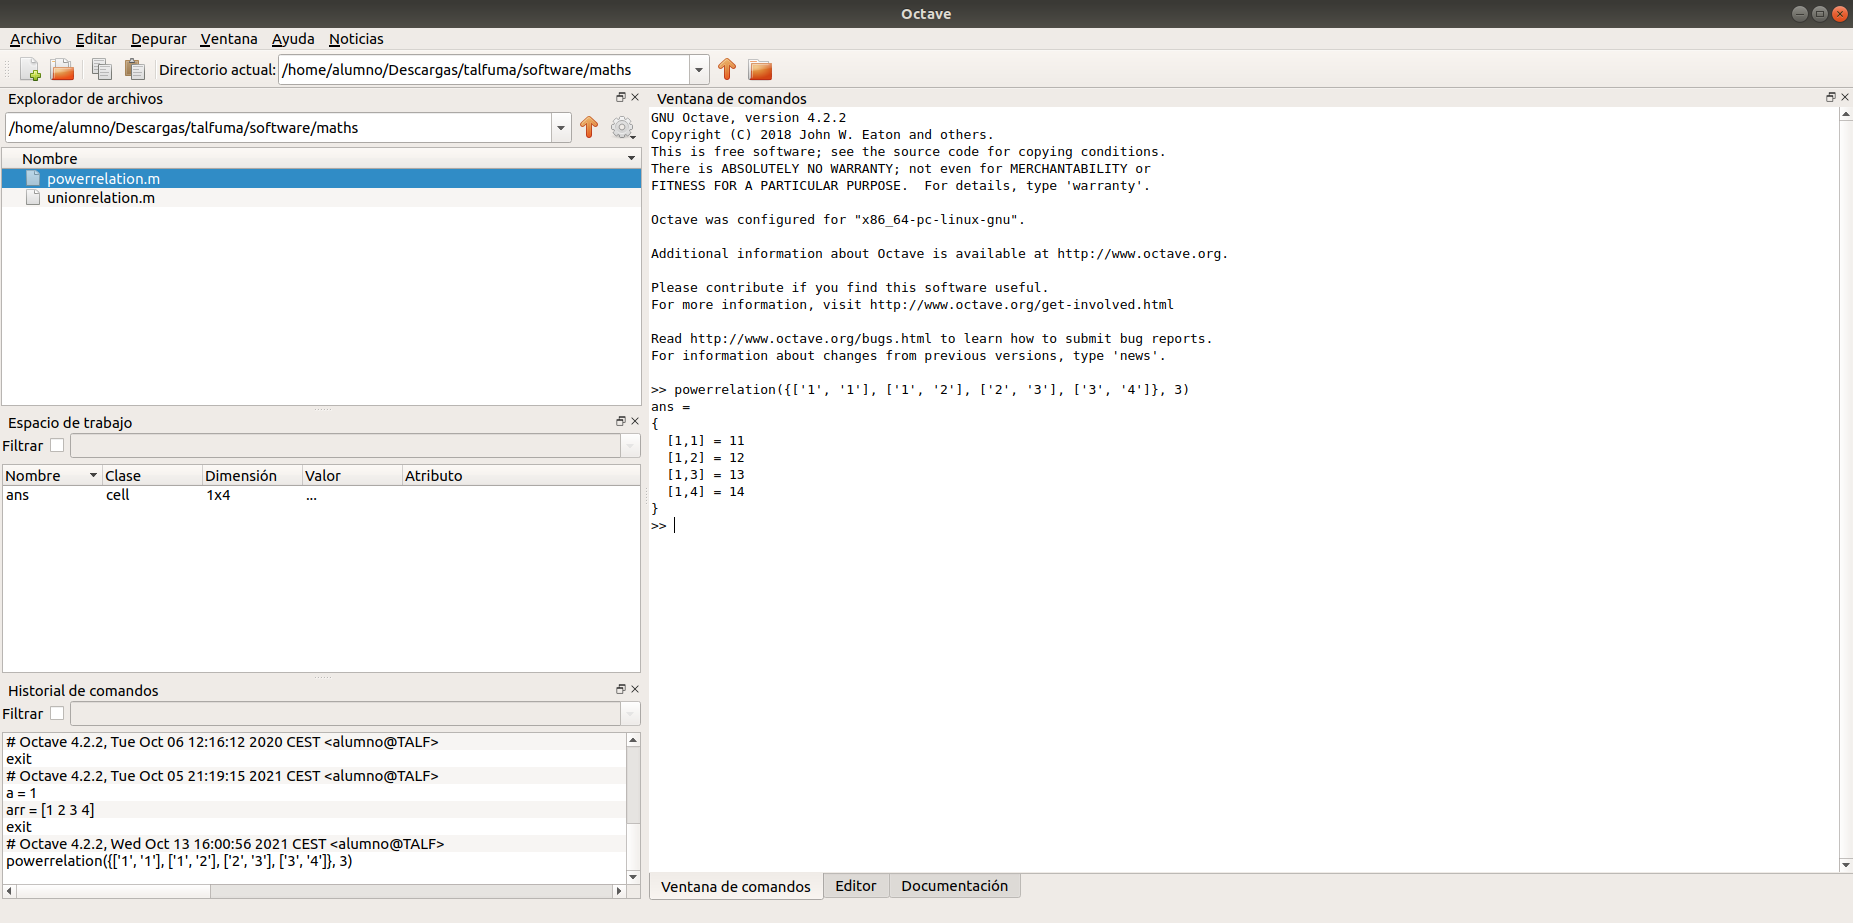
\includegraphics[height=7 cm]{Ejer1.png}

\end{document}
